\begin{question}
Write a concurrent program to multiply two large |n| by |n|
matrices~|a| and~|b| together, storing the result in matrix~|c|.  You should
use the bag-of-tasks pattern.  You should consider what a suitable task
should be: remember that making a task too small will mean that workers spend
most of their time waiting to receive the next task.  \textbf{Optional:} carry
out some experiments to assess different sizes of tasks.
% You will probably want to represent each matrix by a two dimensional array.
% Such an array can be initialised in Scala using, e.g.:
% %
% \begin{scala}
% var a = new Array[Array[Int]](N,N);
% \end{scala}
% %
% The element in position $(i,j)$ can be accessed using \SCALA{a(i)(j)}.
\end{question}

%%%%%%%%%%%%%%%%%%%%%%%%%%%%%%%%%%%%%%%%%%%%%%%%%%%%%%%%%%%%

\begin{answerI}
It would be a mistake to take a task to be the calculation of a \emph{single}
entry in the result matrix.  That would make tasks too small (except, perhaps,
for very large values of~|n|), and lead to the communication channel being a
bottleneck.  Instead, we will take a task to involve calculating
\emph{multiple} entries in the result, |taskSize| entries in the code below.  

However, it's not clear whether a task should be part of a single row, or
multiple rows, i.e.~whether |taskSize| should be smaller or greater than~|n|.
The code below provides for both options: the type |Task| of tasks contains
two subtypes corresponding to the two options.

Most of the code is then straightforward.  Note that each worker can write
values directly into the result matrix~|c|: different threads write to
different entries in~|c| so there are no races.  Both the workers and the
server handle the different types of task in the obvious way.  The main
|apply| function runs the workers and server in parallel, and returns the
result array~|c|.
%
\begin{scala}
class MatrixMult(a: Array[Array[Int]], b: Array[Array[Int]],
             numWorkers: Int, taskSize: Int){
  private val n = a.size

  /** Array to store the result. */
  private var c = Array.ofDim[Int](n,n)

  trait Task

  /** The task to calculate entries £[start..end)£ of row £row£. */
  case class SingleRowTask(row: Int, start: Int, end: Int) extends Task 

  /** The task to calculate rows £[start..end)£. */
  case class MultiRowTask(start: Int, end: Int) extends Task

  /** Channel for sending tasks. */
  private val toWorkers = new SyncChan[Task] // (numWorkers)

  /** Calculate and store entry for £c(i)(j)£. */
  private def calculate(i: Int, j: Int) = {
    var sum = 0; var k = 0
    while(k < n){ sum += a(i)(k)*b(k)(j); k += 1 }
    c(i)(j) = sum
  }

  /** A worker: repeatedly receive tasks, and calculate the relevant rows. */
  private def worker = thread{
    repeat{
      toWorkers?() match{
        case SingleRowTask(row, start, end) =>
          for(j <- start until end) calculate(row,j)
        case MultiRowTask(start, end) => 
          for(row <- start until end){
            var j = 0
            while(j < n){ calculate(row,j); j += 1 }
          }
      }
    }
  }

  private def server = thread{
    if(taskSize <= n){ // use £SingleRowTasks£.
      for(row <- 0 until n){
        var j = 0
        while(j < n){ 
          toWorkers!SingleRowTask(row, j, (j+taskSize) min n); j += taskSize
        }
      }
    }
    else{ // use £MultiRowTasks£.
      assert(taskSize%n == 0); val taskRows = taskSize/n // # rows per task.
      var row = 0
      while(row < n){
        toWorkers!MultiRowTask(row, (row+taskRows) min n); row += taskRows
      }
    }
    toWorkers.endOfStream()
  }

  def apply(): Array[Array[Int]] = {
    run((|| (for(i <- 0 until numWorkers) yield worker)) || server)
    c
  }
}
\end{scala}

%%%%%

Note that the computational cost of calculating each entry is $O(\sm n)$, so
the computational cost of each task is $O(\sm{taskSize} \times \sm n)$, and
the total computational cost is $O(\sm n^3)$.  By contrast, the total
communication cost is $O(\sm n^2 / \sm{taskSize})$.

The graph below gives the results of experiments to investigate the optimal
task size, using eight workers.  Each plot considers a particular value
of~|n|.  The x-axis considers different values for |taskSize| (with
$\sm{taskSize} \le \sm n^2$).  Each observation corresponds to $2^{21}/\sm n$
runs (this means, for a fixed value of |taskSize|, all plots have the same
communication cost).  The plots show the average time taken, with 95\%
confidence intervals, based on 50 observations.

\begin{center}
\begin{tikzpicture}
\begin{semilogxaxis}[
  ylabel = Time (ms),
  xlabel = Task size,
  log basis x=2,
  scaled ticks = false,
  legend pos = north west,
  ymax = 8000,
  height = 0.5\textheight,
  width = 0.8\textwidth
]
\addplot+[error bars/.cd, y dir=both,y explicit] coordinates {
  (16,3411.7514569200002) +- (0,13.35314203117615)
  (32,2069.33146884) +- (0,10.729978495813548)
  (64,1580.71169698) +- (0,12.187170381822089)
  (128,1331.7445018800001) +- (0,17.81049749071006)
  (256,1221.0753941199998) +- (0,14.036122865702522)
  (512,1200.1545826400002) +- (0,13.160170805411989)
  (1024,1224.52603058) +- (0,12.339814224799099)
  (2048,1180.51058504) +- (0,12.667749687921726)
  (4096,1238.1937666600002) +- (0,11.654862280558184)
};
\addlegendentry{$\sm n = 64$}
\addplot+[error bars/.cd, y dir=both,y explicit] coordinates {
  (16,2699.50312402) +- (0,12.525706223272508)
  (32,1492.46816324) +- (0,8.03041925064032)
  (64,1032.61340322) +- (0,9.65428666125068)
  (128,756.41274536) +- (0,9.451155367592488)
  (256,646.3791983) +- (0,8.007846740099064)
  (512,594.56514858) +- (0,8.834111329197311)
  (1024,574.4690993400001) +- (0,8.980969587496622)
  (2048,587.2721347) +- (0,8.86446678781081)
  (4096,592.8091398400001) +- (0,7.043147786939348)
  (8192,676.76904946) +- (0,6.514321066104861)
  (16384,896.66442712) +- (0,4.2726105430776595)
};
\addlegendentry{$\sm n = 128$}
\addplot+[error bars/.cd, y dir=both,y explicit] coordinates {
  (16,2585.2257487600004) +- (0,11.025475452786623)
  (32,1453.85767052) +- (0,8.03717703953275)
  (64,940.0082984) +- (0,6.807915846715892)
  (128,717.61791462) +- (0,9.03977554288971)
  (256,639.46824744) +- (0,9.995634498856198)
  (512,592.3433037799999) +- (0,8.50628975282786)
  (1024,562.1977136) +- (0,7.709808376242314)
  (2048,553.12491324) +- (0,9.561884603261213)
  (4096,557.26886086) +- (0,8.93908705796671)
  (8192,571.2262493200001) +- (0,10.331566458075345)
  (16384,618.6170808200001) +- (0,5.81423301764652)
  (32768,996.1779111000001) +- (0,5.534110197737152)
  (65536,1722.08606682) +- (0,4.427802338996753)
};
\addlegendentry{$\sm n = 256$}
\addplot+[error bars/.cd, y dir=both,y explicit] coordinates {
  (16,2466.5310879) +- (0,8.021048467527224)
  (32,1390.06749204) +- (0,8.237182191779926)
  (64,1193.3307740999999) +- (0,8.065081349160302)
  (128,1041.83938486) +- (0,9.241447251536886)
  (256,969.39207408) +- (0,8.718048838577854)
  (512,1035.4622452) +- (0,12.5560843960807)
  (1024,980.3836694400001) +- (0,10.649524436650921)
  (2048,922.15102602) +- (0,7.74849490705983)
  (4096,877.32535494) +- (0,5.03604122432872)
  (8192,868.437988) +- (0,6.90018903825376)
  (16384,874.77921678) +- (0,10.862135162173832)
  (32768,888.6167595) +- (0,12.722619106651159)
  (65536,1330.923144) +- (0,4.437714457552873)
  (131072,2488.52878918) +- (0,6.620712760530837)
  (262144,4814.394726979999) +- (0,12.967601048815668)
};
\addlegendentry{$\sm n = 512$}
\addplot+[error bars/.cd, y dir=both,y explicit] coordinates {
  (16,4369.8677981) +- (0,48.43900584396743)
  (32,3811.24042716) +- (0,21.672831073712185)
  (64,3882.9536471799997) +- (0,51.87991076642813)
  (128,3681.15564338) +- (0,27.973773946739687)
  (256,3752.1128576399997) +- (0,34.894632015903824)
  (512,3718.3242032) +- (0,25.092378003392046)
  (1024,3635.46097236) +- (0,26.3584784344136)
  (2048,3610.70516356) +- (0,16.29905651068537)
  (4096,3646.10937956) +- (0,30.033869221792447)
  (8192,3648.31660216) +- (0,19.710488335609607)
  (16384,3648.17540688) +- (0,20.541525935467135)
  (32768,3647.67361718) +- (0,21.210072979394173)
  (65536,3600.34809498) +- (0,33.545055491515576)
  (131072,3631.2190203) +- (0,29.952943406403094)
  (262144,6670.03208056) +- (0,38.08685982978708)
  (524288,12716.23585172) +- (0,76.26448592060504)
};
\addlegendentry{$\sm n = 1024$}
\end{semilogxaxis}
\end{tikzpicture}

\end{center}

Each of the plots has a fairly flat middle section, where the value of
|taskSize| makes little difference.  Typically, the fastest behaviour is where
each worker performs a few tasks; but the differences are often smaller than
the confidence intervals, so it's not possible to say definitively.  For most 
values of |n|, particularly small ones, this corresponds to a task being
several rows. 

To the left, the program gets slower, as the communication cost dominates.
This is less of an issue when $\sm n = 1024$, because the computational cost
of each task is still quite large.

To the right, for most values of~|n|, the program gets slower as the number of
tasks is less than the number of workers!  However, for $\sm n = 64$, there is
little difference, as the savings on communication costs roughly balance the
extra computational cost for the workers that receive a task. 
\end{answerI}

%% It makes sense to define a \emph{task} to be the creation of several rows of
%% the result, say \SCALA{taskSize} rows.  
%% % The communication overhead is
%% % $\Theta(n/taskSize)$, so for large arrays, having a task as a single row
%% % (i.e.\ taking $taskSize=1$) would probably be too small a task (although the
%% % communication overhead of using a single row would be reasonably small
%% % compared to the $\Theta(N^3)$ computational cost).  
%% Taking a task to be a single entry in the result would be too small a task: it
%% would give a $\Theta(n^2)$ communication overhead.  Using a whole number of
%% rows (or columns) is easier to program than any other way of splitting up the
%% problem (e.g.\ into square regions).

%% There is no need for the workers to return any result to the controller: each
%% worker can write directly into the result array.  Note that since the tasks
%% write to disjoint parts of the result array, there are no race conditions. 

%% Here's my code:
%% %
%% \begin{scala}
%% class Matrix(a: Array[Array[Int]], b: Array[Array[Int]],
%%              numWorkers: Int, taskSize: Int){
%%   private val n = a.size

%%   /** Array to store the result. */
%%   private var c = Array.ofDim[Int](n,n)

%%   /** A task.  The pair (start,end) represents the task of calculating rows
%%     * [start..end). */
%%   private type Task = (Int,Int) 

%%   /** Channel for sending tasks. */
%%   private val toWorkers = new BuffChan[Task](numWorkers)

%%   /** A worker: repeatedly receive tasks, and calculate the relevant rows. */
%%   private def worker = thread{
%%     repeat{
%%       val(start,end) = toWorkers?()
%%       for(i <- start until end; j <- 0 until n){
%%         // Calculate value for c(i)(j)
%%         var sum = 0
%%         for(k <- 0 until n) sum += a(i)(k)*b(k)(j)
%%         c(i)(j) = sum
%%       }
%%     }
%%   }

%%   /** The controller: repeatedly allocate tasks of size taskSize. */
%%   private def controller = thread{
%%     var current = 0
%%     while(current < n){
%%       toWorkers!(current, current+taskSize min n)
%%       current += taskSize
%%     }
%%     toWorkers.endOfStream
%%   }

%%   /** calculate the product of a and b. */
%%   def apply(): Array[Array[Int]] = {
%%     val system = || (for(w <- 0 until numWorkers) yield worker) || controller
%%     run(system)
%%     c
%%   }
%% }
%% \end{scala}


%% %
%% %% \begin{scala}
%% %% class Matrix(a: Array[Array[Int]], b: Array[Array[Int]], numWorkers: Int, taskSize: Int){
%% %%   private val n = a.size

%% %%   /** Array to store the result. */
%% %%   private var c = Array.ofDim[Int](n,n)

%% %%   /** A task.  The pair (start,end) represents the task of calculating rows [start..end). */
%% %%   private type Task = (Int,Int) 

%% %%   /** Channel for sending tasks. */
%% %%   private val toWorkers = OneMany[Task]

%% %%   /** A worker: repeatedly receive tasks, and calculate the relevant rows. */
%% %%   private def worker = proc{
%% %%     repeat{
%% %%       val(start,end) = toWorkers?()
%% %%       for(i <- start until end; j <- 0 until n){
%% %% 	// Calculate value for c(i)(j)
%% %% 	var sum = 0
%% %% 	for(k <- 0 until n) sum += a(i)(k)*b(k)(j)
%% %% 	c(i)(j) = sum
%% %%       }
%% %%     }
%% %%   }

%% %%   /** The controller: repeatedly allocate tasks of size taskSize. */
%% %%   private def controller = proc{
%% %%     var current = 0
%% %%     while(current < n){
%% %%       toWorkers!(current, current+taskSize min n)
%% %%       current += taskSize
%% %%     }
%% %%     toWorkers.close
%% %%   }

%% %%   /** calculate the product of a and b. */
%% %%   def apply(): Array[Array[Int]] = {
%% %%     run(|| (for(w <- 0 until numWorkers) yield worker) || controller)
%% %%     c
%% %%   }
%% %% }
%% %% \end{scala}

%% %% I ran some informal experiments based around the following function.  The
%% %% ``warm up'' part is to avoid the effects of JIT compilation.
%% %% %
%% %% \begin{scala}
%% %%   /** Measure times for different task sizes, for matrices of size n and
%% %%     * numWorkers worker threads. */
%% %%   def timingTest(n: Int, numWorkers: Int) = {
%% %%     // # reps; chosen to spend ~3s per task size
%% %%     val reps = (300L*Million*numWorkers/(n.toLong*n*n)).toInt
%% %%     println("reps = "+reps)
%% %%     // Warm up
%% %%     for(_ <- 0 until reps){
%% %%       val a = randomArray(n); val b = randomArray(n)
%% %%       val c = new Matrix(a, b, numWorkers, 2)()
%% %%     }
%% %%     println("starting")
%% %%     for(taskSize <- 1 until 10){
%% %%       var elapsed = 0L
%% %%       for(_ <- 0 until reps){
%% %%         val a = randomArray(n); val b = randomArray(n)
%% %%         val start = System.nanoTime
%% %%         val c = new Matrix(a, b, numWorkers, taskSize)()
%% %%         elapsed += System.nanoTime-start
%% %%       }
%% %%       println(taskSize+"\t"+elapsed/Million+"ms")
%% %%     }
%% %%   }
%% %% \end{scala}
%% %

%% I ran some informal experiments, considering different values of~|n|, and
%% different task sizes.
%% For small values of |n| (around 200) a task size of 2 was often best; with
%% smaller tasks, the $O(\sm n^2/\sm{taskSize})$ communication overhead meant
%% that the controller was a bottleneck.  For larger values of |n|, a task size
%% of~1 was best; each task has $O(\sm n^2)$ computational cost, which is
%% sufficiently large that the controller is not a bottleneck; and having more
%% tasks gives better load balancing.  It might be interesting to run experiments
%% with smaller tasks, say to calculate part of a row of the result.
%% \end{answer}
